%!TEX root = main.tex

The evaluation and results of the metrics defined in section~\ref{cap:sec4} is presented in this section. We highlight the most useful metrics, however a previous and complete statistical analysis of the variables in the dataset have been performed. I.e., over 93\% of the BNI attempts are coming from China, more than 90\% of the requests were done via GET method,etc.

\subsection{BN propagation}
In figure~\ref{fig:agg_grow} we can see the aggregate growth of unique IP addresses per day. As we can see, the number of IPs used to try propagate the BN(s) increments daily. Even when we know that ISPs use dynamic IP allocation and therefore, by itself it is not Personal-identifiable information (PII), this metric provide a rough idea of the BNI success and of the size of the problem that is being faced.
Similarly, figure~\ref{fig:bnia_att_d} presents the number of unique IP per day and figure~\ref{fig:bnia_att_i} show the BNI attempts or BN activity in terms of number of requests per day. To compute the relation between this two metrics we have performed a Person's correlation resulting on a 0.5, suggesting that this two analysis are \textit{strongly correlated}~\cite{pear_corr}. Consequently, the growth of the BN is strongly correlated with the increment of attacks, thus, or the BNI is succeeding and/or the BN activity is increasing and with this informations an interested party could motivate the investment on security countermeasures.

\begin{figure}[h]
    \caption{BN growth}
    \label{fig:agg_grow}
    \centering
    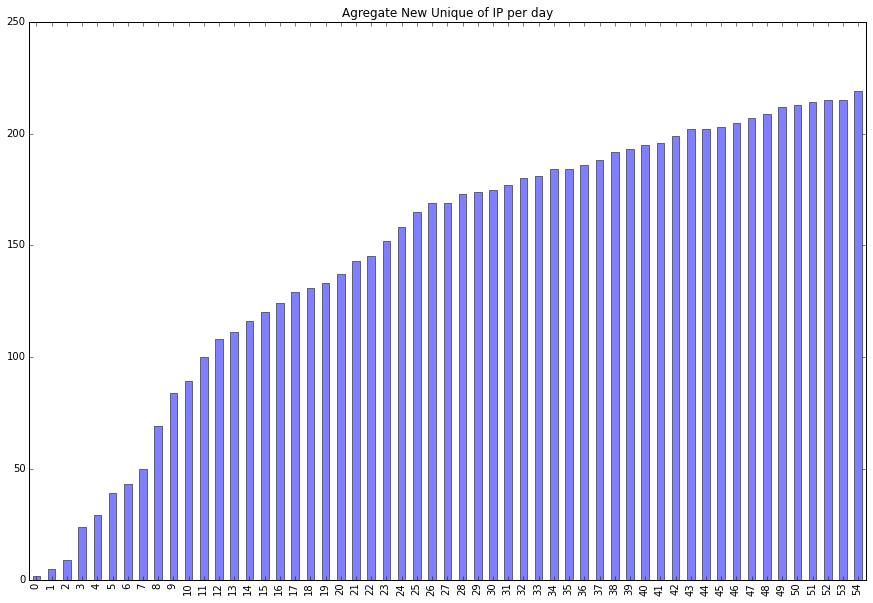
\includegraphics[width=\linewidth]{images/a_new_ip_da}
\end{figure}


\begin{figure*}[ht]
    \begin{subfigure}[ht]{0.5\linewidth}
        \caption{Unique IP per day}
        \label{fig:bnia_att_d}
        \centering
        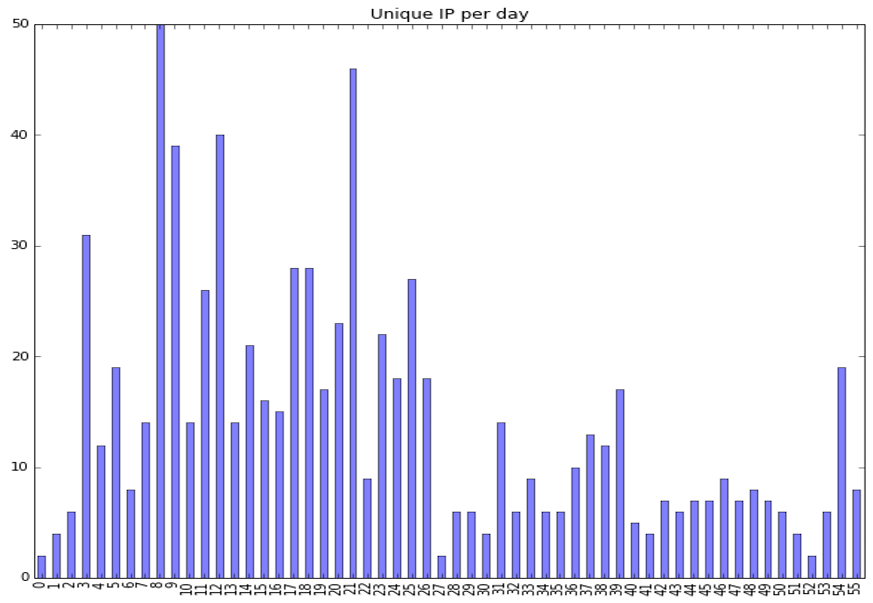
\includegraphics[width=\textwidth]{images/uni_ip_day}
    \end{subfigure}
\quad
    \begin{subfigure}[ht]{0.5\textwidth}
        \caption{BNI attempts}
        \label{fig:bnia_att_i}
        \centering
        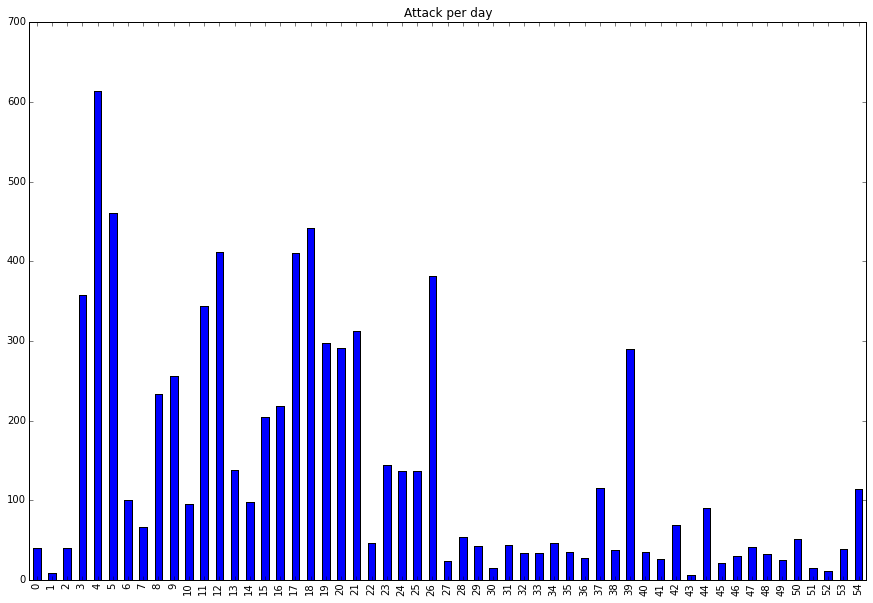
\includegraphics[width=\linewidth]{images/att_day}
    \end{subfigure}

\end{figure*}


\subsection{Network infection radio}
An example of this kind of analysis is shown in figure~\ref{fig:subnet}, we list all the infected IPs in a subnetwork of an ISP, i.e. we have assumed that the ISP has class B IPs and one of his subnetwork is 218.10.0.0. Therefore, for each subnetwork within an ISP network we can see the activity of infected IPs and the infection radio of the subscribers in this network. Further analysis can be done by the ISP since he can use other data sources to get PII from the IPs and therefore compute this metric in a more accurate fashion.

\begin{figure}[h]
    \caption{Subnet 218.10.0.0 attacks}
    \label{fig:subnet}
    \centering
    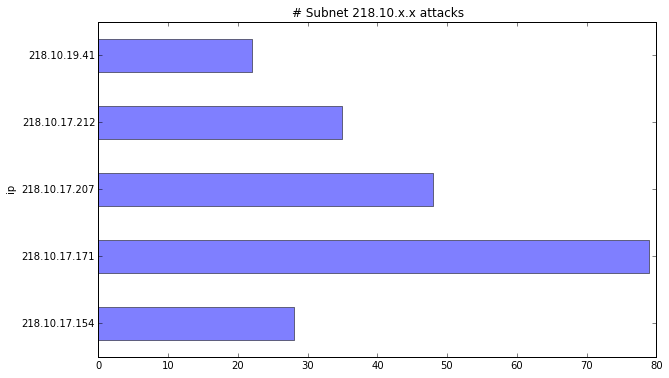
\includegraphics[width=0.9\linewidth]{images/subnet}
\end{figure}

\subsection{BN geographical and digital location.}
Geographical and digital location analysis is shown in figures~\ref{fig:map} and ~\ref{fig:isp}. In figure ~\ref{fig:map} we show the geographical distribution of the BNI attempts

\begin{figure*}[ht]

\caption{BNI geolocation~\cite{map}}
\label{fig:map}
\centering
    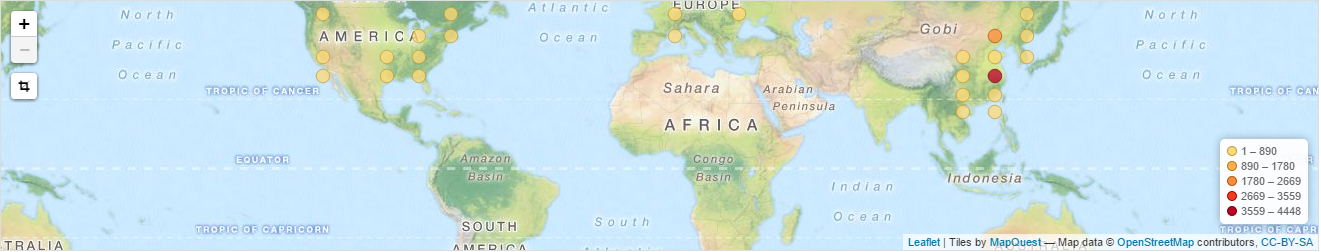
\includegraphics[width=0.9\linewidth]{images/map}
\end{figure*}


% TODO mention IPS data
\begin{figure*}[ht]
\caption{ISP analysis}
\label{fig:isp}
    \begin{subfigure}[ht]{0.5\linewidth}
        \caption{Infected IPs per ISP}
        \label{fig:isp_ip}
    \centering
    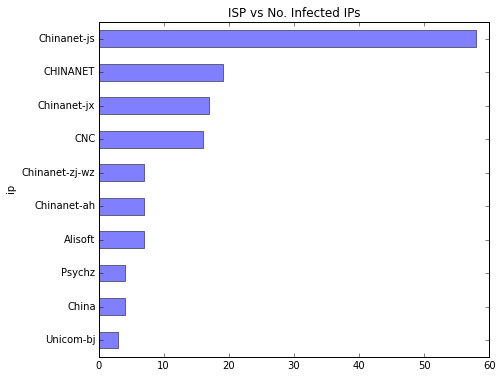
\includegraphics[width=\linewidth]{images/isp_no_ip}
    \end{subfigure}
\quad
    \begin{subfigure}[ht]{0.5\textwidth}
    \caption{BNI attempts per ISP}
    \label{fig:isp_att}
    \centering
    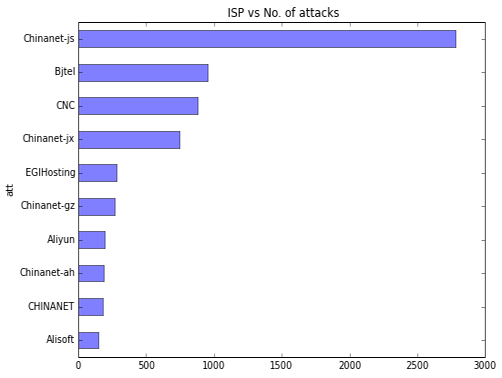
\includegraphics[width=\linewidth]{images/isp_no_att}
    \end{subfigure}

\end{figure*}
